\documentclass{article}
\usepackage[utf8]{inputenc}
\usepackage{fullpage}
\usepackage{amsmath}
\usepackage{tikz}
\usetikzlibrary{trees}
\usepackage{venndiagram}











\begin{document}





% Set the overall layout of the tree
\tikzstyle{level 1}=[level distance=3.5cm, sibling distance=7.5cm]
\tikzstyle{level 2}=[level distance=3.5cm, sibling distance=3cm]

% Define styles for bags and leafs
\tikzstyle{bag} = [text width=4em, text centered]
\tikzstyle{end} = [circle, minimum width=3pt,fill, inner sep=0pt]

\begin{tikzpicture}[grow=right, sloped]
\node[bag] {Urn $3G, 4R, 2W$}
    child {
        node[bag] {$2G, 4R, 2W$}        
            child {
                node[end, label=right: {$P(G_1\cap G_2)=\frac{1}{3}\times\frac{1}{4}=\frac{1}{12}$}] {}
                edge from parent
                node[above] {$G$}
                node[below]  {$\frac{1}{4}$}
            }
            child {
                node[end, label=right: {$P(G_1\cap R_2)=\frac{1}{3}\times\frac{1}{2}=\frac{1}{6}$}] {}
                edge from parent
                node[above] {$R$}
                node[below]  {$\frac{1}{2}$}
            }
            child {
                node[end, label=right: {$P(G_1\cap W_2)=\frac{1}{3}\times\frac{1}{4}=\frac{1}{12}$}] {}
                edge from parent
                node[above] {$W$}
                node[below]  {$\frac{1}{4}$}
            }
            edge from parent 
            node[above] {$G$}
            node[below]  {$\frac{1}{3}$}
    }
    child {
        node[bag] {$3G, 3R, 2W$}   
            child {
                node[end, label=right: {$P(R_1\cap G_2)=\frac{4}{9}\times\frac{3}{8}=\frac{2}{5}$}] {}
                edge from parent
                node[above] {$G$}
                node[below]  {$\frac{3}{8}$}
            }
            child {
                node[end, label=right: {$P(R_1\cap R_2)=\frac{4}{9}\times\frac{3}{8}=\frac{4}{15}$}] {}
                edge from parent
                node[above] {$R$}
                node[below]  {$\frac{3}{8}$}
            }
            child {
                node[end, label=right: {$P(R_1\cap W_2)=\frac{4}{9}\times\frac{1}{4}=\frac{4}{15}$}] {}
                edge from parent
                node[above] {$W$}
                node[below]  {$\frac{1}{4}$}
            }
            edge from parent 
            node[above] {$R$}
            node[below]  {$\frac{4}{9}$}
    }
    child {
        node[bag] {$3G, 4R, 1W$}   
            child {
                node[end, label=right: {$P(W_1\cap G_2)=\frac{2}{9}\times\frac{3}{8}=\frac{1}{12}$}] {}
                edge from parent
                node[above] {$G$}
                node[below]  {$\frac{3}{8}$}
            }
            child {
                node[end, label=right: {$P(W_1\cap R_2)=\frac{2}{9}\times\frac{1}{2}=\frac{1}{9}$}] {}
                edge from parent
                node[above] {$R$}
                node[below]  {$\frac{1}{2}$}
            }
            child {
                node[end, label=right: {$P(W_1\cap W_2)=\frac{2}{9}\times\frac{1}{8}=\frac{1}{36}$}] {}
                edge from parent
                node[above] {$W$}
                node[below]  {$\frac{1}{8}$}
            }
            edge from parent         
            node[above] {$W$}
            node[below]  {$\frac{2}{9}$}
    };
\end{tikzpicture}


\newpage


% Set the overall layout of the tree
\tikzstyle{level 1}=[level distance=3.5cm, sibling distance=5.5cm]
\tikzstyle{level 2}=[level distance=3.5cm, sibling distance=3cm]

% Define styles for bags and leafs
\tikzstyle{bag} = [text width=4em, text centered]
\tikzstyle{end} = [circle, minimum width=3pt,fill, inner sep=0pt]

\begin{tikzpicture}[grow=right, sloped]
\node[bag] {}
    child {
        node[bag] {$\boldsymbol{A'}$}        
            child {
                node[end, label=right: {$\boldsymbol{B'}\ \ \  p(A'\cap B')=p(A')\cdot p(B'|A')$}] {}
                edge from parent
                node[above] {}
                node[below]  {$p(B'|A')$}
            }
            child {
                node[end, label=right: {$\boldsymbol{B}\quad p(A'\cap B)=p(A')\cdot p(B|A')$}] {}
                edge from parent
                node[above] {$p(B|A')$}
                node[below]  {}
            }
            edge from parent 
            node[above] {}
            node[below]  {$p(A')$}
    }
    child {
        node[bag] {$\boldsymbol{A}$}   
            child {
                node[end, label=right: {$\boldsymbol{B'}\quad p(A\cap B')=p(A)\cdot p(B'|A)$}] {}
                edge from parent
                node[above] {}
                node[below]  {$p(B'|A)$}
            }
            child {
                node[end, label=right: {$\boldsymbol{B}\quad p(A\cap B)=p(A)\cdot p(B|A)$}] {}
                edge from parent
                node[above] {$p(B|A)$}
                node[below]  {}
            }
            edge from parent         
            node[above] {$p(A)$}
            node[below]  {}
    };
\end{tikzpicture}

\newpage

% Set the overall layout of the tree
\tikzstyle{level 1}=[level distance=3.5cm, sibling distance=4cm]
\tikzstyle{level 2}=[level distance=3.5cm, sibling distance=2cm]

% Define styles for bags and leafs
\tikzstyle{bag} = [text width=4em, text centered]
\tikzstyle{end} = [circle, minimum width=3pt,fill, inner sep=0pt]

\begin{tikzpicture}[grow=right, sloped]
\node[bag] {$U1$}
    child {
        node[bag] {$\boldsymbol{N1} \to U2:$}        
            child {
                node[end, label=right: {$\boldsymbol{N2}\ \ \  6/25$}] {}
                edge from parent
                node[above] {}
                node[below]  {$3/5$}
            }
            child {
                node[end, label=right: {$\boldsymbol{R2}\quad 4/25$}] {}
                edge from parent
                node[above] {$2/5$}
                node[below]  {}
            }
            edge from parent 
            node[above] {}
            node[below]  {$2/5$}
    }
    child {
        node[bag] { {$\boldsymbol{R1} \to U2:$}}   
            child {
                node[end, label=right: {$\boldsymbol{N2}\quad 9/25$}] {}
                edge from parent
                node[above] {}
                node[below]  {$3/5$}
            }
            child {
                node[end, label=right: {$\boldsymbol{R2}\quad 6/25$}] {}
                edge from parent
                node[above] {$2/5$}
                node[below]  {}
            }
            edge from parent         
            node[above] {$3/5$}
            node[below]  {}
    };
\end{tikzpicture}


\newpage






% Set the overall layout of the tree
\tikzstyle{level 1}=[level distance=3.5cm, sibling distance=7cm]
\tikzstyle{level 2}=[level distance=3.5cm, sibling distance=3.5cm]
\tikzstyle{level 3}=[level distance=3.5cm, sibling distance=2cm]

% Define styles for bags and leafs
\tikzstyle{bag} = [text width=2em, text centered]
\tikzstyle{end} = [circle, minimum width=3pt,fill, inner sep=0pt]

\begin{tikzpicture}[grow=right, sloped]
\node {}
    %******************************************************** RAMA 2
    child {
        node[bag] {$rama2$}  
    %************************************************ RAMA 22
            child {
                node {$rama22$}{}
            		child {
            		node {$hoja222$}
            		edge from parent         
           			node[above] {}
            		node[below]  {$p-hoja222$}
            		}
            		child {
            		node {$hoja221$}
            		edge from parent         
           			node[above] {$p-hoja221$}
            		node[below]  {}
            		}
            		edge from parent         
           			node[above] {}
            		node[below]  {$p-rama22$}
            }
    %************************************************ RAMA 21
            child {
                node {$rama21$}{}
            		child {
            		node {$hoja212$}
            		edge from parent         
           			node[above] {}
            		node[below]  {$p-hoja212$}
            		}
            		child {
            		node {$hoja211$}
            		edge from parent         
           			node[above] {$p-hoja211$}
            		node[below]  {}
            		}
            		edge from parent         
           			node[above] {$p-rama21$}
            		node[below]  {}
            }
            edge from parent         
            node[above] {}
            node[below] {$p-rama2$}
    }
    %******************************************************** RAMA 1
    child {
        node[bag] {$rama1$}   
    %************************************************ RAMA 12
            child {
                node {$rama12$} {}
                	child {
            		node {$hoja122 $}
            		edge from parent         
           			 node[above] {}
            		 node[below]  {$p-hoja122$}
            		}
            		child {
            		node {$hoja121$ }
            		edge from parent         
           			node[above] {$p-hoja121$}
            		node[below]  {}
            		}
            		 edge from parent         
           			 node[above] {}
            		 node[below]  {$p-rama12$}
            }
    %************************************************ RAMA 11
            child {
                node {$rama11$} {}
               		child {
            		node {$hoja112$}
            		edge from parent         
           			node[above] {}
            		node[below]  {$p-hoja112$}
            		}
            		child {
            		node {$hoja111$}
            		edge from parent         
           			node[above] {$p-hoja111$}
            		node[below]  {}
            		}
            		edge from parent         
           			node[above] {$p-rama11$}
            		node[below]  {}
            } 
            edge from parent         
            node[above] {$p-rama1$}
            node[below]  {}
    }
    ;
\end{tikzpicture}



\newpage






% Set the overall layout of the tree
\tikzstyle{level 1}=[level distance=3.5cm, sibling distance=7cm]
\tikzstyle{level 2}=[level distance=3.5cm, sibling distance=3.5cm]
\tikzstyle{level 3}=[level distance=3.5cm, sibling distance=2cm]

% Define styles for bags and leafs
\tikzstyle{bag} = [text width=2em, text centered]
\tikzstyle{end} = [circle, minimum width=3pt,fill, inner sep=0pt]

\begin{tikzpicture}[grow=right, sloped]
\node {}
    %******************************************************** RAMA 2
    child {
        node[bag] {$U2$}  
    %************************************************ RAMA 22
            child {
                node {$N1$}{}
            		child {
            		node {$N2 \to 9/50$}
            		edge from parent         
           			node[above] {}
            		node[below]  {$3/5$}
            		}
            		child {
            		node {$R2 \to 6/50$}
            		edge from parent         
           			node[above] {$2/5$}
            		node[below]  {}
            		}
            		edge from parent         
           			node[above] {}
            		node[below]  {$3/5$}
            }
    %************************************************ RAMA 21
            child {
                node {$R1$}{}
            		child {
            		node {$N2 \to 6/50$}
            		edge from parent         
           			node[above] {}
            		node[below]  {$3/5$}
            		}
            		child {
            		node {$R2 \to 4/50$}
            		edge from parent         
           			node[above] {$2/5$}
            		node[below]  {}
            		}
            		edge from parent         
           			node[above] {$2/5$}
            		node[below]  {}
            }
            edge from parent         
            node[above] {}
            node[below] {$1/2$}
    }
    %******************************************************** RAMA 1
    child {
        node[bag] {$U1$}   
    %************************************************ RAMA 12
            child {
                node {$N1$} {}
                	child {
            		node {$N2 \to 4/50$}
            		edge from parent         
           			 node[above] {}
            		 node[below]  {$2/5$}
            		}
            		child {
            		node {$R2 \to 6/50$ }
            		edge from parent         
           			node[above] {$3/5$}
            		node[below]  {}
            		}
            		 edge from parent         
           			 node[above] {}
            		 node[below]  {$2/5$}
            }
    %************************************************ RAMA 11
            child {
                node {$R1$} {}
               		child {
            		node {$N2 \to 6/60$}
            		edge from parent         
           			node[above] {}
            		node[below]  {$2/5$}
            		}
            		child {
            		node {$R2 \to 9/50$}
            		edge from parent         
           			node[above] {$3/5$}
            		node[below]  {}
            		}
            		edge from parent         
           			node[above] {$3/5$}
            		node[below]  {}
            } 
            edge from parent         
            node[above] {$1/2$}
            node[below]  {}
    }
    ;
\end{tikzpicture}



\newpage



% Set the overall layout of the tree
\tikzstyle{level 1}=[level distance=1.5cm, sibling distance=10cm]
\tikzstyle{level 2}=[level distance=3.5cm, sibling distance=5cm]
\tikzstyle{level 3}=[level distance=6 cm, sibling distance=4cm]

% Define styles for bags and leafs
\tikzstyle{bag} = [text width=2em, text centered]
\tikzstyle{end} = [circle, minimum width=3pt,fill, inner sep=0pt]

\begin{tikzpicture}[grow=right, sloped]
\node {}
    %******************************************************** RAMA 2
    child {
        node[bag] {$B'$}  
    %************************************************ RAMA 22
            child {
                node {$M'$}{}
            		child {
            		node {$L'\quad B'\cap M'\cap L' \to 2/75$}
            		edge from parent         
           			node[above] {$p(L'|B'\cap M')$}
            		node[below]  {$2/5$}
            		}
            		child {
            		node {$L\quad B'\cap M'\cap L \to 3/75$}
            		edge from parent         
           			node[above] {$3/5$}
            		node[below]  {$p(L|B'\cap M')$}
            		}
            		edge from parent         
           			node[above] {$p(M'|B')$}
            		node[below]  {$1/3$}
            }
    %************************************************ RAMA 21
            child {
                node {$M$}{}
            		child {
            		node {$L'\quad B'\cap M\cap L' \to 4/75$}
            		edge from parent         
           			node[above] {$p(L'|B'\cap M)$}
            		node[below]  {$2/5$}
            		}
            		child {
            		node {$L\quad B'\cap M\cap L \to 6/75$}
            		edge from parent         
           			node[above] {$3/5$}
            		node[below]  {$p(L|B'\cap M)$}
            		}
            		edge from parent         
           			node[above] {$2/3$}
            		node[below]  {$P(M|B')$}
            }
            edge from parent         
            node[above] {$p(B')$}
            node[below] {$1/5$}
    }
    %******************************************************** RAMA 1
    child {
        node[bag] {$B$}   
    %************************************************ RAMA 12
            child {
                node {$M'$} {}
                	child {
            		node {$L'\quad B\cap M'\cap L' \to 8/75$}
            		edge from parent         
           			 node[above] {$p(L'|B\cap M')$}
            		 node[below]  {$2/5$}
            		}
            		child {
            		node {$L\quad B\cap M'\cap L \to 12/75$}
            		edge from parent         
           			node[above] {$3/5$}
            		node[below]  {$p(L|B\cap M')$}
            		}
            		 edge from parent         
           			 node[above] {$P(M'|B)$}
            		 node[below]  {$1/3$}
            }
    %************************************************ RAMA 11
            child {
                node {$M$} {}
               		child {
            		node {$L'\quad B\cap M\cap L' \to 16/75$}
            		edge from parent         
           			node[above] {$p(L'|B \cap M)$}
            		node[below]  {$2/5$}
            		}
            		child {
            		node {$L\quad B\cap M\cap L \to 24/75$}
            		edge from parent         
           			node[above] {$3/5$}
            		node[below]  {$p(L|B\cap M)$}
            		}
            		edge from parent         
           			node[above] {$2/3$}
            		node[below]  {$P(M|B)$}
            } 
            edge from parent         
            node[above] {$4/5$}
            node[below]  {$p(B)$}
    }
    ;
\end{tikzpicture}



\newpage


% Set the overall layout of the tree
\tikzstyle{level 1}=[level distance=3cm, sibling distance=2cm]
\tikzstyle{level 2}=[level distance=3cm, sibling distance=1cm]

% Define styles for bags and leafs
\tikzstyle{bag} = [text width=4em, text centered]
\tikzstyle{end} = [circle, minimum width=1pt,fill, inner sep=0pt]

\begin{tikzpicture}[grow=right, sloped]
\node[bag] {}
    child {
        node[bag] {$\boldsymbol{no\ coche}$}        
            child {
                node[end, label=right: {$\boldsymbol{tarde}\quad \ \ 0.18$}] {}
                edge from parent
                node[above] {}
                node[below]  {$0.9$}
            }
            child {
                node[end, label=right: {$\boldsymbol{pronto}\quad 0.02$}] {}
                edge from parent
                node[above] {$0.1$}
                node[below]  {}
            }
            edge from parent 
            node[above] {}
            node[below]  {$0.2$}
    }
    child {
        node[bag] {$\boldsymbol{coche}$}   
            child {
                node[end, label=right: {$\boldsymbol{tarde}\quad \ \ 0.16$}] {}
                edge from parent
                node[above] {}
                node[below]  {$0.2$}
            }
            child {
                node[end, label=right: {$\boldsymbol{pronto}\quad 0.64$}] {}
                edge from parent
                node[above] {$0.8$}
                node[below]  {}
            }
            edge from parent         
            node[above] {$0.8$}
            node[below]  {}
    };
\end{tikzpicture}



\newpage


\vspace{1cm}
\hrule 
\vspace{1cm}

% Set the overall layout of the tree
\tikzstyle{level 1}=[level distance=3cm, sibling distance=2cm]
\tikzstyle{level 2}=[level distance=3cm, sibling distance=1cm]

% Define styles for bags and leafs
\tikzstyle{bag} = [text width=4em, text centered]
\tikzstyle{end} = [circle, minimum width=1pt,fill, inner sep=0pt]

\begin{tikzpicture}[grow=right, sloped]
\node[bag] {}
    child {
        node[bag] {$\boldsymbol{no\ E}$}        
            child {
                node[end, label=right: {$\boldsymbol{-}\quad \ \ 0.9702$}] {}
                edge from parent
                node[above] {}
                node[below]  {$0.98$}
            }
            child {
                node[end, label=right: {$\boldsymbol{+}\quad \ \ 0.0198$}] {}
                edge from parent
                node[above] {$0.02$}
                node[below]  {}
            }
            edge from parent 
            node[above] {}
            node[below]  {$0.99$}
    }
    child {
        node[bag] {$\boldsymbol{E}$}   
            child {
                node[end, label=right: {$\boldsymbol{-}\quad \ \ 0.0003$}] {}
                edge from parent
                node[above] {}
                node[below]  {$0.97$}
            }
            child {
                node[end, label=right: {$\boldsymbol{+}\quad \ \ 0.0097$}] {}
                edge from parent
                node[above] {$0.03$}
                node[below]  {}
            }
            edge from parent         
            node[above] {$0.01$}
            node[below]  {}
    };
\end{tikzpicture}

\vspace{1cm}

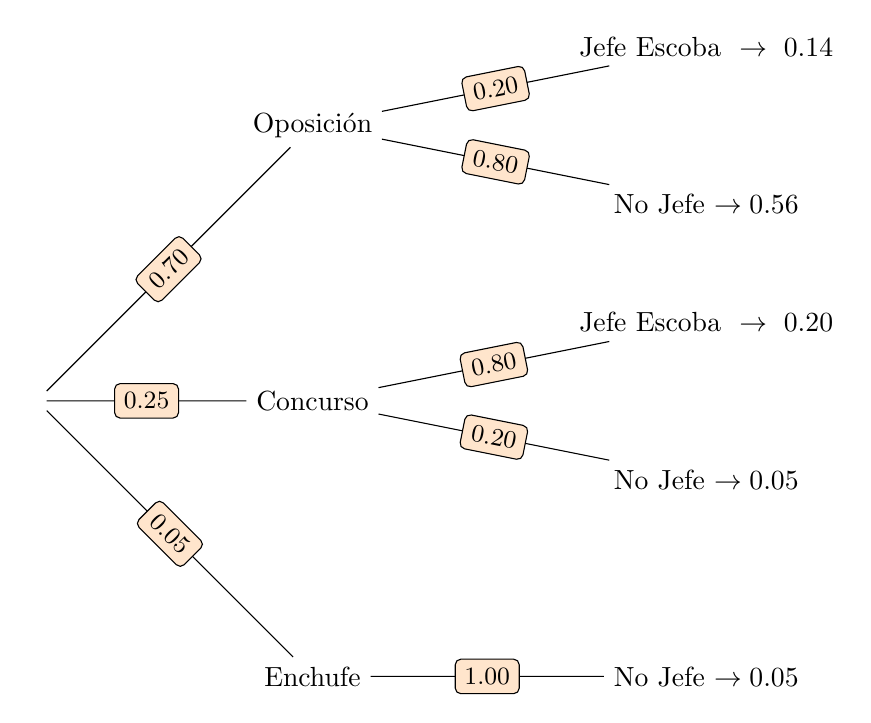
\begin{tikzpicture}[grow=right, sloped]

% Set the overall layout of the tree
\tikzstyle{level 1}=[level distance=3.5cm, sibling distance=3.5cm]
\tikzstyle{level 2}=[level distance=5cm, sibling distance=2cm]


% Define styles for bags and leafs
\tikzstyle{bag} = [text width=4em, text centered]
\tikzstyle{end} = [circle, minimum width=1pt,fill, inner sep=0pt]

%Define probabilidades en naranja con rectángulo negro de bordes redondeados
\tikzstyle{aristas}=[rectangle, rounded corners=2pt, fill=orange!20, draw=black, font=\small]

\node{}
	child{
    	node{Enchufe}
    	child{
    		node{No Jefe $\to 0.05$}
    		edge from parent
    		node[aristas]{$1.00$}
    		}
    	edge from parent
    	node[aristas]{$0.05$}
    }
    child{
    	node{Concurso}
    		child{
    		node{No Jefe $\to 0.05$}
    		edge from parent
    		node[aristas]{$0.20$}
    		}
    		child{
    		node{Jefe Escoba $\ \to \ 0.20$}
    		edge from parent
    		node[aristas]{$0.80$}
    		}
    	edge from parent
    	node[aristas]{$0.25$}
    }
    child{
    	node{Oposición}
    		child{
    		node{No Jefe $\to 0.56$}
    		edge from parent
    		node[aristas]{$0.80$}
    		}
    		child{
    		node{Jefe Escoba $\ \to \ 0.14$}
    		edge from parent
    		node[aristas]{$0.20$}
    		}
    	edge from parent
    	node[aristas]{$0.70$}
    }
	;
\end{tikzpicture}

\newpage


\vspace{2cm}

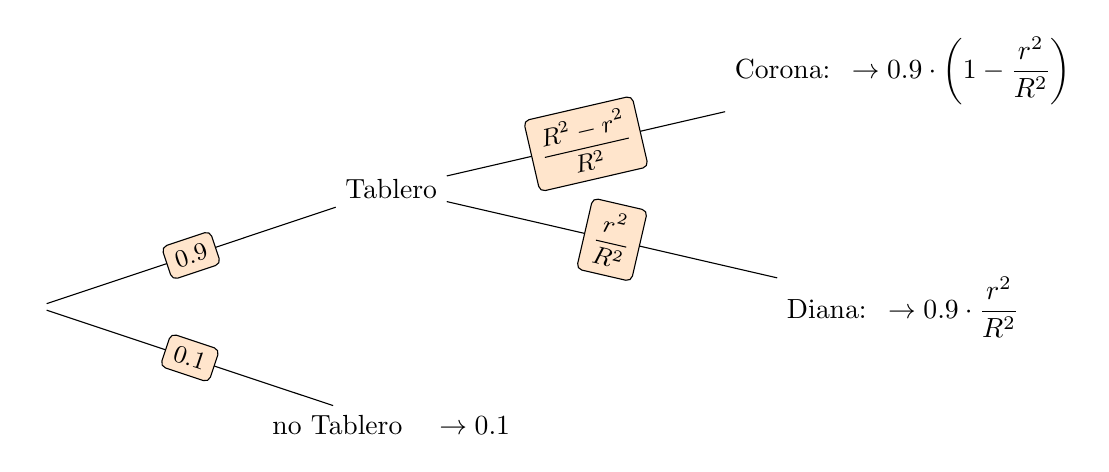
\begin{tikzpicture}[grow=right, sloped]

% Set the overall layout of the tree
\tikzstyle{level 1}=[level distance=4.5cm, sibling distance=3cm]
\tikzstyle{level 2}=[level distance=6.5cm, sibling distance=3cm]


% Define styles for bags and leafs
\tikzstyle{bag} = [text width=4em, text centered]
\tikzstyle{end} = [circle, minimum width=1pt,fill, inner sep=0pt]

%Define probabilidades en naranja con rectángulo negro de bordes redondeados
\tikzstyle{aristas}=[rectangle, rounded corners=2pt, fill=orange!20, draw=black, font=\small]

\node{}
    child{
    	node{no Tablero $\quad \to 0.1$}
    	edge from parent
    	node[aristas]{$0.1$}
    }
    child{
    	node{Tablero}
    		child{
    		node{Diana: $\ \to 0.9 \cdot \dfrac{r^2}{R^2}$}
    		edge from parent
    		node[aristas]{$\dfrac {r^2}{R^2}$}
    		}
    		child{
    		node{Corona: $\ \to 0.9 \cdot \left( 1- \dfrac{r^2}{R^2} \right) $}
    		edge from parent
    		node[aristas]{$\dfrac {R^2-r^2}{R^2}$}
    		}
    	edge from parent
    	node[aristas]{$0.9$}
    }
	;
\end{tikzpicture}



\vspace{3cm}

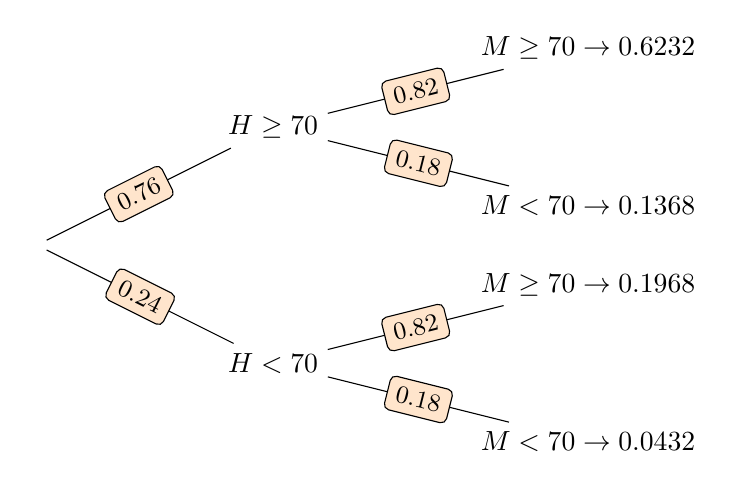
\begin{tikzpicture}[grow=right, sloped]

% Set the overall layout of the tree
\tikzstyle{level 1}=[level distance=3cm, sibling distance=3cm]
\tikzstyle{level 2}=[level distance=4cm, sibling distance=2cm]


% Define styles for bags and leafs
\tikzstyle{bag} = [text width=4em, text centered]
\tikzstyle{end} = [circle, minimum width=1pt,fill, inner sep=0pt]

%Define probabilidades en naranja con rectángulo negro de bordes redondeados
\tikzstyle{aristas}=[rectangle, rounded corners=2pt, fill=orange!20, draw=black, font=\small]

\node{}
    child{
    	node{$H<70$}
    		child{
    		node{$M<70 \to 0.0432$}
    		edge from parent
    		node[aristas]{$0.18$}
    		}
    		child{
    		node{$M\ge 70 \to 0.1968$}
    		edge from parent
    		node[aristas]{$0.82$}
    		}
    	edge from parent
    	node[aristas]{$0.24$}
    }
    child{
    	node{$H\ge 70$}
    		child{
    		node{$M<70 \to 0.1368$}
    		edge from parent
    		node[aristas]{$0.18$}
    		}
    		child{
    		node{$M\ge 70 \to 0.6232$}
    		edge from parent
    		node[aristas]{$0.82$}
    		}
    	edge from parent
    	node[aristas]{$0.76$}
    }
	;
\end{tikzpicture}


\begin{table}[]
\centering
\begin{tabular}{c|c|c|c}
\cline{2-3}
\textbf{} & \textbf{$H\ge 70$} & \textbf{$H<70$} & \textbf{} \\ \hline
\multicolumn{1}{|c|}{\textbf{$M\ge 70$}} & 0.6232 & 0.1968 & \multicolumn{1}{c|}{\textbf{0.82}} \\ \hline
\multicolumn{1}{|c|}{\textbf{$M<70$}} & 0.1368 & 0.0432 & \multicolumn{1}{c|}{\textbf{0.18}} \\ \hline
\textbf{} & \textbf{0.76} & \textbf{0.24} & \textbf{} \\ \cline{2-3}
\end{tabular}
\end{table}



\newpage

PRUEBA Vídeo

\vspace{2cm}



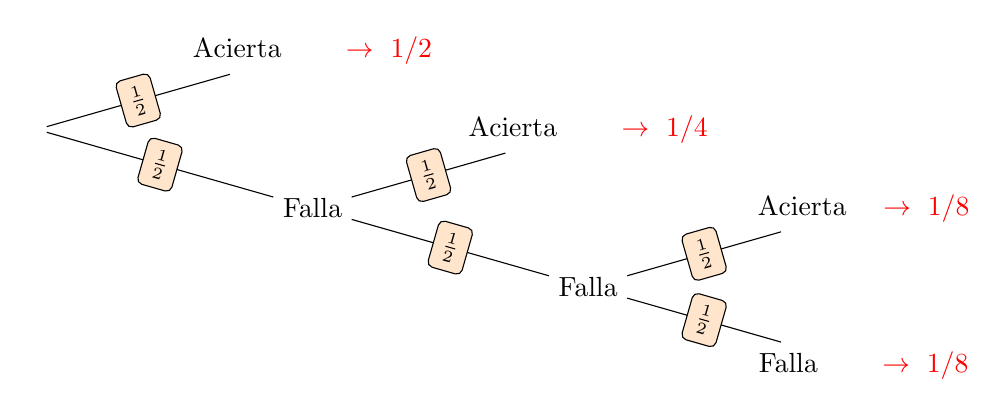
\begin{tikzpicture}[grow=right, sloped]

% Set the overall layout of the tree
\tikzstyle{level 1}=[level distance=3.5cm, sibling distance=2cm]
\tikzstyle{level 2}=[level distance=3.5cm, sibling distance=2cm]
\tikzstyle{level 3}=[level distance=3.5cm, sibling distance=2cm]

% Define styles for bags and leafs
\tikzstyle{bag} = [text width=4em, text centered]
\tikzstyle{end} = [circle, minimum width=1pt,fill, inner sep=0pt]

%Define probabilidades en naranja con rectángulo negro de bordes redondeados
\tikzstyle{aristas}=[rectangle, rounded corners=2pt, fill=orange!20, draw=black, font=\small]

\node{}
    child{
   		node{Falla}
   			child{
   				node{Falla}
   					child{
   						node{Falla $\qquad \textcolor{red}{\to \ 1/8}$}
   						edge from parent
    					node[aristas]{$\frac 1 2$}
    				}
    				child{
    					node{Acierta $\quad \textcolor{red}{\to \ 1/8}$}
    					edge from parent
    					node[aristas]{$\frac 1 2$}
    				}
    			edge from parent
    			node[aristas]{$\frac 1 2$}
   			 }
   		 	child{
    			node{Acierta $\qquad \textcolor{red}{\to \ 1/4}$}
    			edge from parent
    			node[aristas]{$\frac 1 2$}
   			 }
   		edge from parent
    	node[aristas]{$\frac 1 2$}
    }
    child{
    	node{Acierta $\qquad \textcolor{red}{\to \ 1/2}$}
    	edge from parent
    	node[aristas]{$\frac 1 2$}
    }
    ;  
\end{tikzpicture}

\vspace{2cm}



\begin{center}
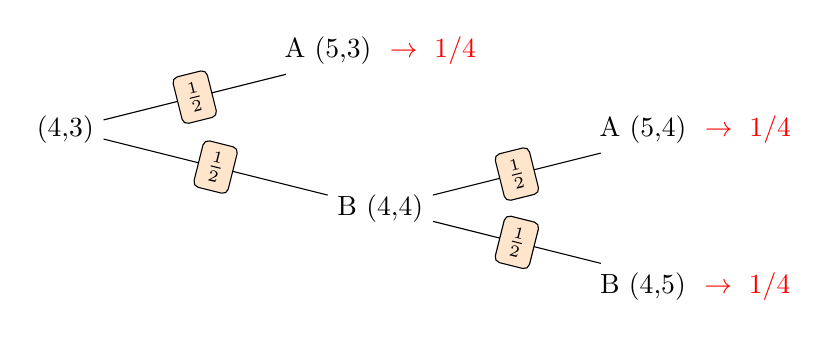
\begin{tikzpicture}[grow=right, sloped]

% Set the overall layout of the tree
\tikzstyle{level 1}=[level distance=4cm, sibling distance=2cm]
\tikzstyle{level 2}=[level distance=4cm, sibling distance=2cm]


% Define styles for bags and leafs
\tikzstyle{bag} = [text width=4em, text centered]
\tikzstyle{end} = [circle, minimum width=1pt,fill, inner sep=0pt]

%Define probabilidades en naranja con rectángulo negro de bordes redondeados
\tikzstyle{aristas}=[rectangle, rounded corners=2pt, fill=orange!20, draw=black, font=\small]

\node{(4,3)}
    child{
   		node{B (4,4)}
   			child{
   				node{B (4,5) $\ \textcolor{red}{\to \ 1/4}$}
    			edge from parent
    			node[aristas]{$\frac 1 2$}
   			 }
   		 	child{
    			node{A (5,4) $\ \textcolor{red}{\to \ 1/4}$}
    			edge from parent
    			node[aristas]{$\frac 1 2$}
   			 }
   		edge from parent
    	node[aristas]{$\frac 1 2$}
    }
    child{
    	node{A (5,3) $\ \textcolor{red}{\to \ 1/4}$}
    	edge from parent
    	node[aristas]{$\frac 1 2$}
    }
    ;  
\end{tikzpicture}
\end{center}

\newpage







%************************************************************************
\newpage
\section{Diagramas de Venn}






\begin{venndiagram2sets}
\fillA	
\end{venndiagram2sets}
No funciona multicols. bklac dnksc. D ÑDSH cdusi guisd UIO  nskjahjkdhk.  cdsc ldsc dsdsah jdsh sds ss DUsdlugs. hj hfdsjk. hfd svhjvjhfdj fjdvjklsvdh vjkdhv bklac dnksc. D ÑDSH cdusi guisd UIO  nskjahjkdhk.  cdsc ldsc dsdsah jdsh sds ss DUsdlugs. hj hfdsjk. hfd svhjvjhfdj fjdvjklsvdh vjkdhvbklac dnksc. D ÑDSH cdusi guisd UIO  nskjahjkdhk.  cdsc ldsc dsdsah jdsh sds ss DUsdlugs. hj hfdsjk. hfd svhjvjhfdj fjdvjklsvdh vjkdhv bklac dnksc. D ÑDSH cdusi guisd UIO  nskjahjkdhk.  cdsc ldsc dsdsah jdsh sds ss DUsdlugs. hj hfdsjk. hfd svhjvjhfdj fjdvjklsvdh vjkdhvbklac dnksc. D ÑDSH cdusi guisd UIO  nskjahjkdhk.  cdsc ldsc dsdsah jdsh sds ss DUsdlugs. hj hfdsjk. hfd svhjvjhfdj fjdvjklsvdh vjkdhv


\vspace{1cm}


\begin{venndiagram2sets}
\fillACapB	
\end{venndiagram2sets}

\vspace{1cm}

\begin{venndiagram2sets}
\fillNotA	
\end{venndiagram2sets}

\vspace{1cm}

\begin{venndiagram2sets}
\fillNotAorB	
\end{venndiagram2sets}

\vspace{1cm}

\begin{venndiagram3sets}
\fillACapBNotC	
\end{venndiagram3sets}


\vspace{1cm}

\begin{venndiagram3sets}[labelA=Eco, labelB=Mat, labelC=Len, labelOnlyA=1, labelOnlyB=2, labelOnlyC=3, labelABC=7, labelOnlyAB=4, labelOnlyAC=5, labelOnlyBC=6, tikzoptions={scale=2, font=\Large, draw=red}]
	
\end{venndiagram3sets}


\vspace{1cm}





\vspace{1cm}

\begin{venndiagram3sets}[labelA=Eco, labelB=Mat, labelC=Len, labelOnlyA=1, labelOnlyB=2, labelOnlyC=3, labelABC=7,  labelOnlyAB=4, labelOnlyAC=5, labelOnlyBC=6,  tikzoptions={scale=2, font=\Large, draw=red}]

	\fillA
	
\end{venndiagram3sets}




\vspace{1cm}

\begin{venndiagram3sets}[shade=orange!10,labelA=Eco, labelB=Mat, labelC=Len, labelOnlyA=1, labelOnlyB=2, labelOnlyC=3, labelABC=7, labelOnlyAB=4, labelOnlyAC=5, labelOnlyBC=6, tikzoptions={scale=2, font=\Large, draw=red}]

	\fillACapBNotC % Solo A y B
	\fillNotABC    % Fuera 
	
	
\end{venndiagram3sets}

\newpage

\begin{center}
Tabla de la función de distribución $\Phi$ de una normal $N(0,1)$ para $x\geq 0$

    $$
    \Phi(x)=P[X\leq x]=\frac{1}{\sqrt{2\pi}}\int_{-\infty}^x\exp\left(\frac{-t^2}{2}\right)\,dt
    $$
    
    Si $x<0\ \Rightarrow \  \Phi(x)=1-\Phi(-x)$
\end{center}

$\quad$

\begin{center}
\begin{footnotesize}
\begin{tabular}{|r|rrrrrrrrrr|}\hline
\textbf{N(0,1)} & 0.00 & 0.01 & 0.02 & 0.03 & 0.04 & 0.05 & 0.06 & 0.07 & 0.08 & 0.09 \\ \hline
0.0 & 0.500000 & 0.503989 & 0.507978 & 0.511966 & 0.515953 & 0.519939 & 0.523922 & 0.527903 & 0.531881 & 0.535856 \\
0.1 & 0.539828 & 0.543795 & 0.547758 & 0.551717 & 0.555670 & 0.559618 & 0.563559 & 0.567495 & 0.571424 & 0.575345 \\
0.2 & 0.579260 & 0.583166 & 0.587064 & 0.590954 & 0.594835 & 0.598706 & 0.602568 & 0.606420 & 0.610261 & 0.614092 \\
0.3 & 0.617911 & 0.621720 & 0.625516 & 0.629300 & 0.633072 & 0.636831 & 0.640576 & 0.644309 & 0.648027 & 0.651732 \\
0.4 & 0.655422 & 0.659097 & 0.662757 & 0.666402 & 0.670031 & 0.673645 & 0.677242 & 0.680822 & 0.684386 & 0.687933 \\
0.5 & 0.691462 & 0.694974 & 0.698468 & 0.701944 & 0.705401 & 0.708840 & 0.712260 & 0.715661 & 0.719043 & 0.722405 \\
0.6 & 0.725747 & 0.729069 & 0.732371 & 0.735653 & 0.738914 & 0.742154 & 0.745373 & 0.748571 & 0.751748 & 0.754903 \\
0.7 & 0.758036 & 0.761148 & 0.764238 & 0.767305 & 0.770350 & 0.773373 & 0.776373 & 0.779350 & 0.782305 & 0.785236 \\
0.8 & 0.788145 & 0.791030 & 0.793892 & 0.796731 & 0.799546 & 0.802337 & 0.805105 & 0.807850 & 0.810570 & 0.813267 \\
0.9 & 0.815940 & 0.818589 & 0.821214 & 0.823814 & 0.826391 & 0.828944 & 0.831472 & 0.833977 & 0.836457 & 0.838913 \\
1.0 & 0.841345 & 0.843752 & 0.846136 & 0.848495 & 0.850830 & 0.853141 & 0.855428 & 0.857690 & 0.859929 & 0.862143 \\
1.1 & 0.864334 & 0.866500 & 0.868643 & 0.870762 & 0.872857 & 0.874928 & 0.876976 & 0.879000 & 0.881000 & 0.882977 \\
1.2 & 0.884930 & 0.886861 & 0.888768 & 0.890651 & 0.892512 & 0.894350 & 0.896165 & 0.897958 & 0.899727 & 0.901475 \\
1.3 & 0.903200 & 0.904902 & 0.906582 & 0.908241 & 0.909877 & 0.911492 & 0.913085 & 0.914657 & 0.916207 & 0.917736 \\
1.4 & 0.919243 & 0.920730 & 0.922196 & 0.923641 & 0.925066 & 0.926471 & 0.927855 & 0.929219 & 0.930563 & 0.931888 \\
1.5 & 0.933193 & 0.934478 & 0.935745 & 0.936992 & 0.938220 & 0.939429 & 0.940620 & 0.941792 & 0.942947 & 0.944083 \\
1.6 & 0.945201 & 0.946301 & 0.947384 & 0.948449 & 0.949497 & 0.950529 & 0.951543 & 0.952540 & 0.953521 & 0.954486 \\
1.7 & 0.955435 & 0.956367 & 0.957284 & 0.958185 & 0.959070 & 0.959941 & 0.960796 & 0.961636 & 0.962462 & 0.963273 \\
1.8 & 0.964070 & 0.964852 & 0.965620 & 0.966375 & 0.967116 & 0.967843 & 0.968557 & 0.969258 & 0.969946 & 0.970621 \\
1.9 & 0.971283 & 0.971933 & 0.972571 & 0.973197 & 0.973810 & 0.974412 & 0.975002 & 0.975581 & 0.976148 & 0.976705 \\
2.0 & 0.977250 & 0.977784 & 0.978308 & 0.978822 & 0.979325 & 0.979818 & 0.980301 & 0.980774 & 0.981237 & 0.981691 \\
2.1 & 0.982136 & 0.982571 & 0.982997 & 0.983414 & 0.983823 & 0.984222 & 0.984614 & 0.984997 & 0.985371 & 0.985738 \\
2.2 & 0.986097 & 0.986447 & 0.986791 & 0.987126 & 0.987455 & 0.987776 & 0.988089 & 0.988396 & 0.988696 & 0.988989 \\
2.3 & 0.989276 & 0.989556 & 0.989830 & 0.990097 & 0.990358 & 0.990613 & 0.990863 & 0.991106 & 0.991344 & 0.991576 \\
2.4 & 0.991802 & 0.992024 & 0.992240 & 0.992451 & 0.992656 & 0.992857 & 0.993053 & 0.993244 & 0.993431 & 0.993613 \\
2.5 & 0.993790 & 0.993963 & 0.994132 & 0.994297 & 0.994457 & 0.994614 & 0.994766 & 0.994915 & 0.995060 & 0.995201 \\
2.6 & 0.995339 & 0.995473 & 0.995604 & 0.995731 & 0.995855 & 0.995975 & 0.996093 & 0.996207 & 0.996319 & 0.996427 \\
2.7 & 0.996533 & 0.996636 & 0.996736 & 0.996833 & 0.996928 & 0.997020 & 0.997110 & 0.997197 & 0.997282 & 0.997365 \\
2.8 & 0.997445 & 0.997523 & 0.997599 & 0.997673 & 0.997744 & 0.997814 & 0.997882 & 0.997948 & 0.998012 & 0.998074 \\
2.9 & 0.998134 & 0.998193 & 0.998250 & 0.998305 & 0.998359 & 0.998411 & 0.998462 & 0.998511 & 0.998559 & 0.998605 \\
3.0 & 0.998650 & 0.998694 & 0.998736 & 0.998777 & 0.998817 & 0.998856 & 0.998893 & 0.998930 & 0.998965 & 0.998999 \\
3.1 & 0.999032 & 0.999065 & 0.999096 & 0.999126 & 0.999155 & 0.999184 & 0.999211 & 0.999238 & 0.999264 & 0.999289 \\
3.2 & 0.999313 & 0.999336 & 0.999359 & 0.999381 & 0.999402 & 0.999423 & 0.999443 & 0.999462 & 0.999481 & 0.999499 \\
3.3 & 0.999517 & 0.999534 & 0.999550 & 0.999566 & 0.999581 & 0.999596 & 0.999610 & 0.999624 & 0.999638 & 0.999651 \\
3.4 & 0.999663 & 0.999675 & 0.999687 & 0.999698 & 0.999709 & 0.999720 & 0.999730 & 0.999740 & 0.999749 & 0.999758 \\
3.5 & 0.999767 & 0.999776 & 0.999784 & 0.999792 & 0.999800 & 0.999807 & 0.999815 & 0.999822 & 0.999828 & 0.999835 \\
3.6 & 0.999841 & 0.999847 & 0.999853 & 0.999858 & 0.999864 & 0.999869 & 0.999874 & 0.999879 & 0.999883 & 0.999888 \\
3.7 & 0.999892 & 0.999896 & 0.999900 & 0.999904 & 0.999908 & 0.999912 & 0.999915 & 0.999918 & 0.999922 & 0.999925 \\
3.8 & 0.999928 & 0.999931 & 0.999933 & 0.999936 & 0.999938 & 0.999941 & 0.999943 & 0.999946 & 0.999948 & 0.999950 \\
3.9 & 0.999952 & 0.999954 & 0.999956 & 0.999958 & 0.999959 & 0.999961 & 0.999963 & 0.999964 & 0.999966 & 0.999967 \\
4.0 & 0.999968 & 0.999970 & 0.999971 & 0.999972 & 0.999973 & 0.999974 & 0.999975 & 0.999976 & 0.999977 & 0.999978 \\
\hline
\end{tabular}
\end{footnotesize}
\end{center}

\newpage



\end{document}
